\chapter{Hierarchical Multiple Instance learning} \label{chap:hmill}
The goal of this thesis is to use specifically hierarchical multiple instance learning (\emph{hmill}) for classification. Using it we want to follow the prior art in this area \cite{Mandlik2020} where author pointed out elegant way to classify \emph{JSON} documents. In comparison to GNN approach \emph{hmill} model has better scalability \cite{Mandlik2020} which is convenient for our \emph{JSON reports}. In this chapter we describe multiple instance learning as generalization of standard learning approach described in previous chapter. Then we describe \emph{hmill} framework, which we use.

% In this chapter we describe multiple instance learning as extended approach compared to previus chapter. In the second part we will describe hierarchical multiple instance learning framework as modelling tool to model tree-structured data. Finally, we will address its usage in malware classification and other applications in cyber security field.

\section{Multiple instance learning}
At first let us describe and define problem of \emph{Multiple instance learning} its origin and formalism. This term firstly appeared in \citet{Dietterich1997}, it is not the very first formulation of such problem, that is in \cite{Keeler1991}.

The motivation example in original paper \cite{Dietterich1997} is formulated in following way. Imagine we have keys and some of them unlock specific door and some of them not (no other choice). Important is that we do not have access to the door. In standard learning is our goal to learn classification model which consumes key and outputs if it is able to open the door or not. But in \emph{multiple instance learning} setting we receive whole key chains (with various number of keys) and without checking every single key we have to classify if the whole chain is able to open the door.

In the figure \ref{fig:mill} we can see basic idea behind \emph{Mill} problem. The only significant change regarding previous chapter is definition of \emph{Example}. 
\paragraph{Example}
We assume \emph{supervised} learning setting. Our examples consist of two parts - \emph{bag} $$b$$ and \emph{state} $$y$$. State was defined earlier and its meaning is the same but it is related to bag and sometimes called \emph{bag label}. \emph{Bag} $$b$$ is set of feature vectors $$x_i$$, these vectors are called \emph{instances} and usually lives in standard feature space $$x_i \in \mathbb{R}^{d}$$. Cardinality of each bag $$|b| \in \mathbb{N}$$ and can be even zero. We assume that $$b \in \mathcal{B}$$ which denotes \emph{bag space}. \emph{Bag space} might also be seen as $$\mathcal{B} = \mathrm{Fin}(\mathcal{X})$$ which denotes all finite subsets of $$\mathcal{X}$$. Now we can see that standard learning situation described in chapter \ref{chap:classification} is just \emph{Mill} problem where holds $$|b| = 1$$.

For the purposes of our thesis we assume mill classification problem so $$|\mathcal{Y}|$$ is finite (typically binary classification $$\mathcal{Y} \in \{positive, negative\}$$). 
% Some researches and even the original paper has one assumption (sometimes called \emph{Standard assumption}). This assumption is about underlying \emph{instance labels} and their relation to \emph{bag labels}. This assumptions is often relaxed \cite{Xu2003} and that is also our case.

\begin{figure}
    \centering
    \begin{subfigure}{.5\textwidth}
      \centering
        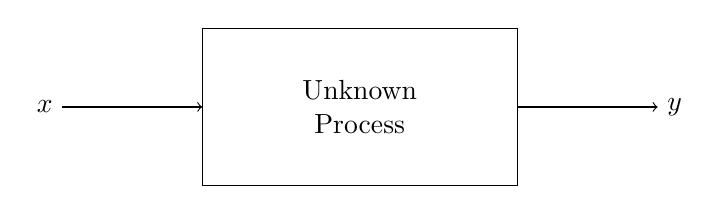
\begin{tikzpicture}
            \node (X) at (-2,1) {$x$};
            \node (Y) at (6,1) {$y$};
            \draw (0,0)rectangle(4,2)node[midway,black,align=center]{Unknown \\ Process};
            \path [->] (X) edge (0,1);
            \path [->] (4,1) edge (Y);
        \end{tikzpicture}
      \caption{Standard situation}
    \end{subfigure}%
    \begin{subfigure}{.5\textwidth}
      \centering
        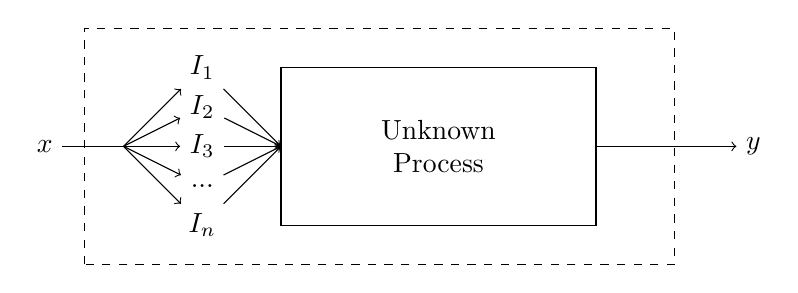
\begin{tikzpicture}
            \node (X) at (-3,1) {$x$};
            \node (Y) at (6,1) {$y$};
            \node (I1) at (-1,2) {$I_1$};
            \node (I2) at (-1,1.5) {$I_2$};
            \node (I3) at (-1,1) {$I_3$};
            \node (I4) at (-1,0.5) {$...$};
            \node (I5) at (-1,0) {$I_n$};
            \draw (0,0)rectangle(4,2)node[midway,black,align=center]{Unknown \\ Process};
            
            \path [-] (X) edge (-2,1);
            \path [->] (-2,1) edge (I1);
            \path [->] (-2,1) edge (I2);
            \path [->] (-2,1) edge (I3);
            \path [->] (-2,1) edge (I4);
            \path [->] (-2,1) edge (I5);
            \path [->] (I1) edge (0,1);
            \path [->] (I2) edge (0,1);
            \path [->] (I3) edge (0,1);
            \path [->] (I4) edge (0,1);
            \path [->] (I5) edge (0,1);
            \path [->] (4,1) edge (Y);
            
            \draw [dashed] (-2.5,-0.5)rectangle(5,2.5);
        \end{tikzpicture}
      \caption{Multiple instance situation}
    \end{subfigure}
    \caption{Supervised learning}
    \label{fig:mill}
\end{figure}


\begin{figure}[!ht]
    \centering
    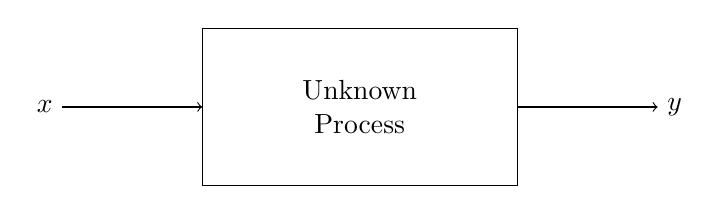
\begin{tikzpicture}
        \node (X) at (-2,1) {$x$};
        \node (Y) at (6,1) {$y$};
        \draw (0,0)rectangle(4,2)node[midway,black,align=center]{Unknown \\ Process};
        \path [->] (X) edge (0,1);
        \path [->] (4,1) edge (Y);
    \end{tikzpicture}
    \caption{Graphs of three analytical functions.}
    \label{fig:analytical}
\end{figure}

\begin{figure}[!ht]
    \centering
    
    \caption{Graphs of three analytical functions.}
    \label{fig:analytical}
\end{figure}

% \todo{I have to mention some citations the theory I built on top of Mandlik and Amores!}
% \todo{image of standard setting vs mill setting} \todo{if we would like to have some fancy figure we can try something with keys}

\section{Solving of \emph{Mill} problems}
The goal is the same regardless the standard or multiple instasnce setting, we would like to find discriminative modelling approach to be able to solve classification task. Three general approaches (paradigms) to solve \emph{mill} problems are formulted in \cite{Amores2013} - \emph{Instance-Space, Bag-Space} and \emph{Embedded-Space} paradigm.

\subsection{Instance-Space paradigm}
An algorithm in this group infers \emph{instance-based} classifier $f(x) \in \{1,0\}$ for each instance in training set. \emph{Bag-based} classifier is constructed in following way - $F(b)=\frac{f(x_1)\circ f(x_2)\circ\dots\circ f(x_N)}{Z}$, where $x_i$ are instances in bag $b$, $\circ$ denotes an algorithm-specific aggregation operator and $Z$ denotesa an optional normalization factor. As we stated earlier \emph{bag labels} are part of training but not \emph{instance labels}, which means methods using this paradigm have to make some assumptions about the relation between \emph{bag} and \emph{instance} labels.
\subsubsection{Standard assumption}
Our assumption is that each negative bag consists of negative instances only and each positive bag includes at least one positive instance. The goal of algorithm in this setup is to aim at instances that make bags positive (we know that at least one in each bag does that).

There are several methods which follow this assumption. First is \emph{Axis-Parallel Rectangle} used in \cite{Dietterich1997} in drug discovery use case, where $F(b)=\max_{x\in b}f(x)$. Other methods are \emph{Diverse Density} \cite{Maron1998} or MI-SVM \cite{Andrews2003}.

\subsubsection{Collective assumption}
Previous methods tend to look over the fact that the bag labels might be influenced by the interaction of instance features. For example in learning stage some of them might consider only several instances (or even one) from the whole bag.

\emph{Collective assumption} states that \quote{all instances in a bag contribute equally to the bag’s label} \cite{Xu2003}. Methods usualy use training set of instances which is constructed such that each instance inherits label from bag where it is is presented. This training set might by used to get instance-level classifier. Basic approach is applying SIL algorithm \cite{Bunescu2007}, which simply train mentioned instance-level classifier and bag-level classifier is obtained by $F(b)=\frac{1}{|b|}\sum_{x\in b}f(x)$. Other method is Wrapper MI \cite{Frank2003}.


\subsection{Bag-Space paradigm}
In this setup we treat whole bags to learn classifier. The discriminant learning process is performed in \emph{bag space} directly in contrast to previous paradigm where we assumed instance-level classifiers.

\emph{Bag space} is non-vectorial, we are able to define such distance function $D(b_1,b_2)$, where $b_1$, $b_2$ are bags and the result is representing a measure of their similarity (or distance). This function we can use in standard distance-based classifiers such as SVM or K-NN.

Instances lives in \emph{d-dimensional} spaces, so we can see them as points and then bags are set of points. Example of distance function is minimal Hausdorff distance $D(b_1,b_2)=\min_{x\in b_1, y\in b_2}||x-y||$, which denotes distance between closest points of bags $b_1$ and $b_2$ \cite{Wang2000}. We can also use kernel functions $K(b_1,b_2)$ which provide similarity between bags (set of points). An example of such kernel might be $K(b_1,b_2)=\sum_{x\in b_1, y\in b_2}k(x-y)^{p}$, where $k(x,y)$ denotes instance-level kernel (linear, polynomial\dots) and $p$ is related to size of the largest bag (in practise found by cross validation) \cite{Gartner2002}.

\subsection{Embedded-Space paradigm}
In Bag-Space paradigm the goal is to extract global information from bags, this is achieved by defining distance function which allow us their implicit comparison. In Embedded-Space paradigm we extract the information by defining explicit mapping $\mathcal{M}:b\mapsto v$ from the bag space to custom feature space which summarizes bag characteristics, we call $\mathcal{M}$ embedding. Based on the choice of $\mathcal{M}$ we distinguish two approaches - \emph{without vocabulary} and \emph{vocabulary-based} methods.

\emph{Without vocabulary} approaches make no differentiation among instances in bag and aggregates overall statistics from each instance of the bag. Example of such algorithm might be \emph{Simple MI} where the feature vector for bag is attained by averaging over all instances in it - $\mathcal{M}(b)=\frac{1}{|b|}\sum_{x\in b}x$ \cite{Dong2006}.

\subsubsection{Vocabulary-based methods}
These methods are still in embedded-space category and main idea is to find an embedding based on instance-level classfication. However, classes are taken in difference sense than in Instance-Space paradigm, here we often involve an unsupervised way so the semantics of class is missing here. Bag embedding is then determined according to instance classes. These methods are called \emph{vocabulary-based} because we need a vocabulary of all instance-level classes in training set. This vocabulary is used to classify instances.

There are three usual components of \emph{vocalbulary-based method} \cite{Amores2013}. \emph{Vocabulary} $\mathcal{V}$ storing instance level classes (sometimes rather called concepts). Each concepts is defined by identifier and set of parameters. These concepts are most often created from result of K-means algorithm. Second component is \emph{mapping function} $\mathcal{M}(b, \mathcal{V})=v$ (embedding) which is mapping from \emph{bag space} to $k$-dimensional \emph{feature space}, where $k$ denotes number of concepts. Final component of \emph{vocabulary-based method} is standard supervised classifier $\mathcal{G}(v) in \{1,0\}$ which classifies feature vectors in \emph{embedded space}. Final bag-level classifier results in $F(b)=\mathcal{G}(\mathcal{M}(b,\mathcal{V}))$

\subsubsection{Histogram-based methods}
In this sub-paradigm $\mathcal{V}$ denotes resulting clusters of chosen clustering algorithm which outputs $K$ classes $C_1,\dots C_K$. $\mathcal{M}$ denotes histogram of classes in instances in particular bag - $\mathcal{M}(b,\mathcal{V})=(v_1,v_2\dots,v_K)$, where $v_j=\frac{1}{Z}\sum_{x\in b}f_{j}(x), j=1,\dots,K$, where $f_{j}(x) \in \{1,0\}$ is likelihood that instance $x$ belongs to class $C_j$ and $Z$ is normalization factor. Example of algorithm like this is Bag-of-Words \cite{Nowak2006}.

Remainding methods are \emph{Distance-based} and \emph{Attribute-based} methods, for more info we refer to \cite{Amores2013}.

Finally, we arrived at the crux method we are going to use. Great generalization of all paradigms is provided in \cite{Mandlik2020}. Authors stated that all approaches require three components - function operation at the instance level of instances $f$ (e. g. \ class classifier), a form of aggregation or pooling $g$ and bag-level classifier $F$. As this all together might be seen as function composition, we might involve gradient-based optimization, which is the idea of \cite{Pevny2016a, Edwards2017}. As we stated in previous chapter using gradient-based optimization leads us to the requirement that the functions (in this case $f$,$g$ and $F$) have to be (at least piecewise) differentiable with respect to their parameters. This approach is very flexible because we do not have to solve particular interactions of components like in previous cases where they are designed separatedly and later connected. The overall flexibility and expresivity comes from the fact that all the functions and their parameters are optimized together. For more, no instance labels are required, they are treated in unsupervised manner, the bag labels are the only information which is provided. Example of architecture of such neural network is demonstrated in \ref{fig:hmill}. Note that there is one $f$ with shared parameters $\Theta_{f}$ over all instances. The pooling function $g$ might be mean or maximum and final layer $F$ after the pooling uses fixed dimension bag representation.

\begin{figure}[!ht]
    \centering
    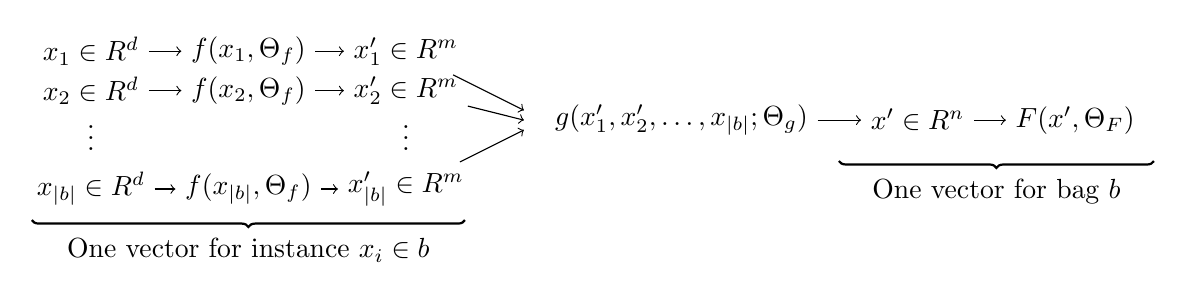
\begin{tikzpicture}
        \node (I1) at (-6,2) {$x_1 \in \mathbb{R}^{d}$};
        \node (I12) at (-4,2) {$f(x_1,\Theta_{f})$};
        \node (I13) at (-2,2) {$x_1' \in \mathbb{R}^{m}$};
        \path[->] (I1) edge (I12);
        \path[->] (I12) edge (I13);
        
        \node (I2) at (-6,1.5) {$x_2 \in \mathbb{R}^{d}$};
        \node (I22) at (-4,1.5) {$f(x_2,\Theta_{f})$};
        \node (I23) at (-2,1.5) {$x_2' \in \mathbb{R}^{m}$};
        \path[->] (I2) edge (I22);
        \path[->] (I22) edge (I23);
        
        \node (Ik) at (-6,1) {\vdots};
        \node (Ik3) at (-2,1) {\vdots};
        
        \node (I3) at (-6,0.25) {$x_{|b|} \in \mathbb{R}^{d}$};
        \node (I32) at (-4,0.25) {$f(x_{|b|},\Theta_{f})$};
        \node (I33) at (-2,0.25) {$x_{|b|}' \in \mathbb{R}^{m}$};
        \path[->] (I3) edge (I32);
        \path[->] (I32) edge (I33);
        
        \node (G) at (1.5,1.125) {$g(x_1',x_2',\dots,x_{|b|};\Theta_{g})$};
        \path[->] (I33) edge (-0.5,1);
        \path[->] (I23) edge (-0.5,1.125);
        \path[->] (I13) edge (-0.5,1.25);
        
        \node (R) at (4.5,1.125) {$x' \in \mathbb{R}^{n}$};
        \path[->] (G) edge (R);
        
        \node (F) at (6.5,1.125) {$F(x',\Theta_{F})$};
        \path[->] (R) edge (F);
        
        
        \draw[thick,decorate,decoration={brace, raise=-3pt}] (-1.25, -0.25) -- (-6.75, -0.25) node[midway,below]{One vector for instance $x_i \in b$ };

        \draw[thick,decorate,decoration={brace, raise=-3pt}] (7.5, 0.5) -- (3.5,0.5) node[midway,below]{One vector for bag $b$ };
        
    \end{tikzpicture}
    \caption{Hierarchical mill model by \cite{Pevny2016a} (image inspired by \cite{Mandlik2020})}
    \label{fig:hmill}
\end{figure}

Demonstration of this approach and its results can be found in \cite{Pevny2016a,Pevny2017, PevnyDedic2020, Mandlik2020, Janisch2020,PevnyKovarik2019a}. The same idea was published independently as \emph{Deep sets} by \cite{Zaheer2018}.

In \cite{Mandlik2020} we can see application of this approach in created \emph{hmill} framework and its convincing application for \emph{JSON} documents. Our goal is to use this framework for the \emph{JSON} documents collected during dynamic malware analysis. Further we describe this framework.



% \todo{List paradigm and shortly describe and add some examples (prior) of solutions - cite from Amores}
% another examples we can find here - https://www.etsmtl.ca/Unites-de-recherche/LIVIA/Recherche-et-innovation/Publications/Publications-2017/mil_marc_2017.pdf

% \todo{some real world examples (not only pevny and Mandlik).}


% - Prior experiments (Some of them mention here, some of them below in hmill section)
%     Look at applications which are in previous papers above (mandlik, pevny..)
%         \cite{Stiborek2018}

\section{HMill framework}
The idea of the neural net architecture defined in \cite{Pevny2016a} was followed by \cite{Mandlik2020} which led to formulation of \emph{HMill framework} reffering to \emph{Hierarchical Multiple instance learning framework}. This framework builds on the top of the idea of hierarchically composed models introduced above and provides general tools to create models which structurally follows the data. Both sample and model consist of various type nodes which are structured as rooted directed tree. The crucial publication for \emph{hmill framework} is \cite{Mandlik2020} where authors firstly formulated this framework and demonstrated its use. In this section we summarize the most important facts. Should reader wish to learn more, we recommend original publication \cite{Mandlik2020}.

\subsection{Abstract data nodes}
Firstly, let us summarize basic data nodes in \emph{hmill} framework. Demonstration of the types usage can be seen in figure \ref{fig:irismill}.
\todo{transform figure to pdf}
\subsubsection{Array node}
Our data consists of some low level observations like - strings, booleans, vectors, enums\dots Authors call these raw observations - \emph{fragments} and $\mathcal{F}$ denotes the space where they are living. Examples of $\mathcal{F}$ might be Euclidean space $\mathbb{R}^{k}$, linear space $\mathbb{Z}^{2}$ or even all strings over finite alphabet. The only requirement for $\mathcal{F}$ is that there have to exist such mapping $\mathcal{F}\xleftarrow{h}\mathbb{R}^{n}$. The array node is responsible for storing \emph{fragments} $\alpha\in\mathcal{F}$ in following form: $an(\alpha,\mathcal{F},h)$. Sometimes the notation is $an(x)$, where $x=h(\alpha)$ meaning that the trasformation was already made.

\subsubsection{Bag node}
\emph{Bag node} denotes analogy to \emph{bag} in multipliple instance learning $bn(b)$, where $b=\{a_1,\dots,a_{|b|}\}$. From the structural point of view (tree) bag node can be created if that node has multiple children which are $an$ with matching $\mathcal{F}$ and second case if it has multiple subtrees $bn_i$ with matching (more complex) structure\footnote{follows same schema which is defined later} (nested). As the instances have to be of the same structure they form an unordered set.

\subsubsection{Product node}
Final node type of \emph{hmill} tree representation of sample is \emph{product node}. That is defined as $pn(a_1,\dots,a_{l}$, where $l\geq1$ and $a_i$ is representation of some \emph{hmill} tree/subtree - \emph{an,bn,ps}. The order of $a_i$ is arbitrary but fixed.

\begin{figure}[h]
    \centering
    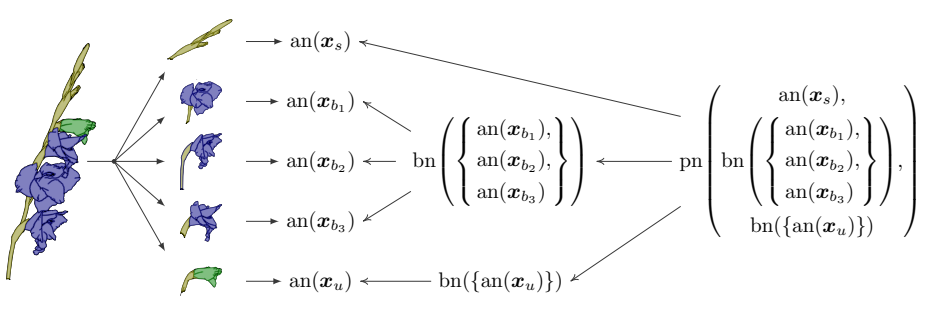
\includegraphics[width=8cm]{figures/irismill.png}
    \caption{Representation of the plant specimen in \emph{Hmill} framwork (source \cite{Mandlik2020})}
    \label{fig:irismill}
\end{figure}

\subsection{HMill schema}
In the \emph{bag node} definition we mentioned that instances in it have to follow same structure. That is why we define \emph{HMill schema}. Schemas are trees which are mirroring sample trees and for each abstract data node there are corresponding information stored in the schema structure. See below.
\begin{itemize}
    \item \emph{Array schema node} ($as(\mathcal{F'},h')$ - defines fragments space instance $\mathcal{F'}$ and mapping $h'$
    \item \emph{Bag schema node} ($bs(s')$) - defines subschema (subtree) of instances $s'$ specifying structure of instance in bag node
    \item \emph{Product schema node} ($ps(s_1,\dots,s_{l})$) - defines one or more subschemata $s_i$ of subtrees in product node
\end{itemize}

\paragraph{Definition} (Schema matching according to \cite{Mandlik2020}). We say that a sample tree $t$ follows a schema $s$, or matches a schema $s$, provided following conditions hold:
\begin{itemize}
    \item If $t=an(\alpha,\mathcal{F},h)$ for any $\alpha\in\mathcal{F}$, then $t$ is matching $s$ if and only if $s=as(\mathcal{F},h)$
    \item If $t=bn(\{a_1,\dots,a_k\})$, then $t$ is matching $s$ if and only if $s=bs(s')$ and $\forall i\in\{1,\dots,k\}:t_i$ matches $s'$
    \item If $t=pn(t_1,\dots,t_l)$, then $t$ is matching $s$ if and only if $s=ps(s_1,\dots,s_k)$,$l=k$ and $\forall i\in\{1,\dots,l\}:t_i$ matches $s_i$
\end{itemize}

Note that empty bag node match every schema with bag node as root, so if we observe two sample following same structure and one of them has instances in specific bag and second does not, they still might follow the same schema.
\subsection{HMill model}
After we defined sample and schema, we are able to treat our dataset and create \emph{hmill} samples $\mathcal{T}$ ready for modelling. Following the idea of the tree structure mirroring in case of schema definition we define \emph{hmill} model in the same manner. The goal here is to create model based on schema extracted from our data, which would accept each sample $s\in\mathcal{T}$ on input. Models are made of model nodes and represent functions. During single sample evaluation using our model, we evaluate subtrees first and lastly their parent. The root provides the model output. The model nodes are hierarchically nested function, each of wich outputs one vector given one sample. All nodes are piecewise differentiable with respect to their input.

\subsubsection{Array model - $am(f)$}
This model trasforms leaves of sample trees. The input of $f$ is in $\mathbb{R}^{m}$ because we assume mapping $h$ is already applied for original fragment. So $f:\mathbb{R}^m\rightarrow\mathbb{R}^n$. We migh use any piecewise differentiable mapping but authors refer to dense, feedforward neural networks.

\subsubsection{Bag model - $bm(f,g,F)$}
\emph{Bag model} is motivated by solution of mill problem provided in \cite{Pevny2016a}. Each bag can be seen as mil solver for the problem defined by corresponding bag node and its instances. Three functions are composed - $f$ denotes \emph{instance model}, $g$ denotes \emph{aggregation} and $F$ denotes \emph{bag mapping}. On each instance/subtree $a_i$ in $bn(a_1,\dots,a_k)$ we apply $f$. All results are input for one or more aggregation functions $g$, its output is a single vector. Finally, the \emph{bag mapping} $F$ is applied. The output lives in from $\mathbb{R}^d$, where $d$ is output dimension of particular multiple instance model. If the bag model is in the root of the tree $d$ is overall dimension of the model, we often use $d=|C|$ as number of classes, the output is then interpreted as logits of probabilities of classes.

$f$ might be arbitrarily complex HMill model accepting HMill tree, its output has to be $\mathbb{R^m}$. Note that all nodes in bag node has to follow same schema so the $f$ is the same for all instances (subtrees) and the output space is of fixed dimension for all subtrees. We might use for instance \emph{max} or \emph{mean} as aggregation function $g$. Authors of framework use one or more layer of a feedforward neural network as $F$.

\subsubsection{Product model - $pm(f_1,\dots,f_l,f_p)$}
Product model consists of $l$ submodels, each processes  one child of a corresponding product data node an one more final mapping $f_p$. Each product data node can follow different schema so each $f_i$ might be different (not like in case of bag model). By applying all $f_i$ to corresponding product nodes we get $l$ vectors which might have different length. Product model concatenate all vector and the result is transformed one or more time by $f_p$.

As all functions in the tree structured model are defined to be at least piecewise differentiable with respect to all parameters the backpropagation algorithm is adopted in the overall model optimization. Its adaptation we can find in \cite{Mandlik2020}.

\todo{maybe add image on page 27 in mandlik...}

% schema and matching schema, valid sample
% Hmill models - try to describe it more briefly and connect it to the original idea by Pevny - do not use many images from mandlik but the original iris and the last one to demonstrate the relation to Pevny, or my simplified version

\subsection{Modelling JSON documents using HMill framework}
Following our goal to model the collected data using \emph{HMill} model we would like to focus specific use case which is modelling \emph{JSON} documents. Original publication \cite{Mandlik2020} contains even such approach and even experimental results for \emph{IoT device identification} use case. In previous chapter we described several approaches for such data classification, now we describe how the \emph{HMill} framework might be used.

Assuming that we have a set of \emph{JSON} documents as dataset $\mathcal{T}$ we require one condition to hold. All documents in our dataset have to follow same structure (same schema) which means following:
\begin{itemize}
    \item Given a fixed position in the tree, we know which keys can be found in this particular position in all documents $d\in\mathcal{T}$.
    \item Values of the same key at the same position in all documents $d\in\mathcal{T}$ must follow same structure.
    \item Arrays at the same position in all documents $d\in\mathcal{T}$ must be empty or contain same structured objects.
\end{itemize}

Note that the document can follow same schema even if it is missing some keys. The condition of matching schema might seem limiting but it is very common setup that documents used for single use case follow the same schema. This is true especially for machine generated documents.

\emph{JSON} to \emph{HMill} sample translation is defined on three basic abstract node types. Each leaf of the tree (JSON primitive data types) are transformed into array node $an(h(\dots))$, $h$ denotes mapping to $\mathbb{R}^n$. Mapping $h$ is the same for all leaves at the same position across the dataset and it might be different for different positions. Product data is used to model \emph{JSON} objects. Because product node accepts an ordered set, the keys in the \emph{JSON} object are ordered. Finally, \emph{JSON} arrays are modelled as bag nodes.

\todo{image of json document in our use case, but the idea is the same like in Mandlik fig 5.4}

Authors of framework mentioned that the model is taking into game even the structure which exceeds the \emph{flattening} approach. Compared to the rule-based approaches, the framework is able to learn more complex hypotheses because chosen aggregation can substitute various hand-defined rules. The \emph{HMill} framework was used in an IoT device identification use case \cite{Mandlik2020} which was a dataset of \emph{JSON} documents in multinomial classification modelling. Reported accuracy was $96$~\%. Authors experimented even in different setup for general graph inference to demonstrate the generality of \emph{HMill} framework.

The conclusion of this chapter and maybe the most significant conslusion for our work is that it is possible to use \emph{HMill framework} to classify tree-structured data e.g. \ \emph{JSON} documents. \citeauthor{Mandlik2020} presents convincing results (for example on \emph{device identification} example) and that is why this framework is directly in assignment of this thesis.

Regardless of quite comprehensive theory which is covered in this part of the thesis, \emph{HMill} framework is still not everything. Our goal is quite cross-cutting and the model we are going to train we want also explain. What we mean by explanation we describe in next chapter.

%---------------------REMAINING-------------------------------------

% HMILL:
% - assumptions - https://en.wikipedia.org/wiki/Multiple_instance_learning (Be aware, I think those are not true all at once...), also algorithm list is presented, could be mentioned, and other interesting references like problem generalization
% - between modern approaches mention adapting of single instance algorithms

% Previous connection
% - We focus on structured data and our tool is hmill, let's describe it
% Way through this chapter
% - multiple instance learning
% - hierarchical mill
% - prior
%     - Prior in various fields
%     - Prior in cybersec
% Next connection
% - Not necessary, but can connect to next chapter slightly (we want to explain this kind of model)

% Stand on Madlik chapter, his citations (be aware), somol and Pevny


% - GOALS 
% - Learn the hierarchical multiple instance learning framework (HMill)
% - describe theory, connect it to classical approach
% - Usual usage of this type of learning - classification, regression...
% - Our usecase and experiments with this kind of learning in malware classification field (prior)